
\chapter{1일차, 한강 상류}
\section{여행의 시작, 태백}
\subsection{이무기가 몸부림 친 곳, 검룡소}
서울을 가르는 거대한 물줄기, 한강은 어디서 시작되었을까? 
강원도 태백에는 1987년 국립지리원에서 인정받은 한강의 공식 발원지 검룡소가 있다. 
검룡소는 강원도 태백시 창죽동 금대봉 산기슭에 위치한다. 
이곳의 이름이 검룡소(儉龍沼)인 까닭은 이곳에 전해내려오는 전설과 관련이 깊다. 과거 서해에는 이무기가 살았다. 
이 이무기는 용이 되기 위해 한강의 강줄기를 거슬러 올라오기 시작했고, 결국 이곳 검룡소에 도착하게 된다. 
이무기가 용이 되기 위해 물이 솟는 굴에 들어가려 몸부림치는 바람에 검룡소 주변 물줄기의 모습이 마치 용틀임하는 것처럼 보이게 되었다고 한다. 

\subsection{한강의 발원지}
검룡소는 해발 800m에 위치해 있으며, 한강 하류까지 총 500km가 넘는 한강의 급수를 담당한다. 
검룡소에서는 사시사철 $9^\circ C$의 차가운 물이 흘러나오며, 
하루에 2,000톤 가량의 물이 굴에서 뿜어져 나와 계곡을 따라 흐른다. 
검룡소에서 시작한 물은 골지천으로 흐르는데, 이 골지천이 한강의 발원천이다. 

\begin{figure}[ht]
    \centering
    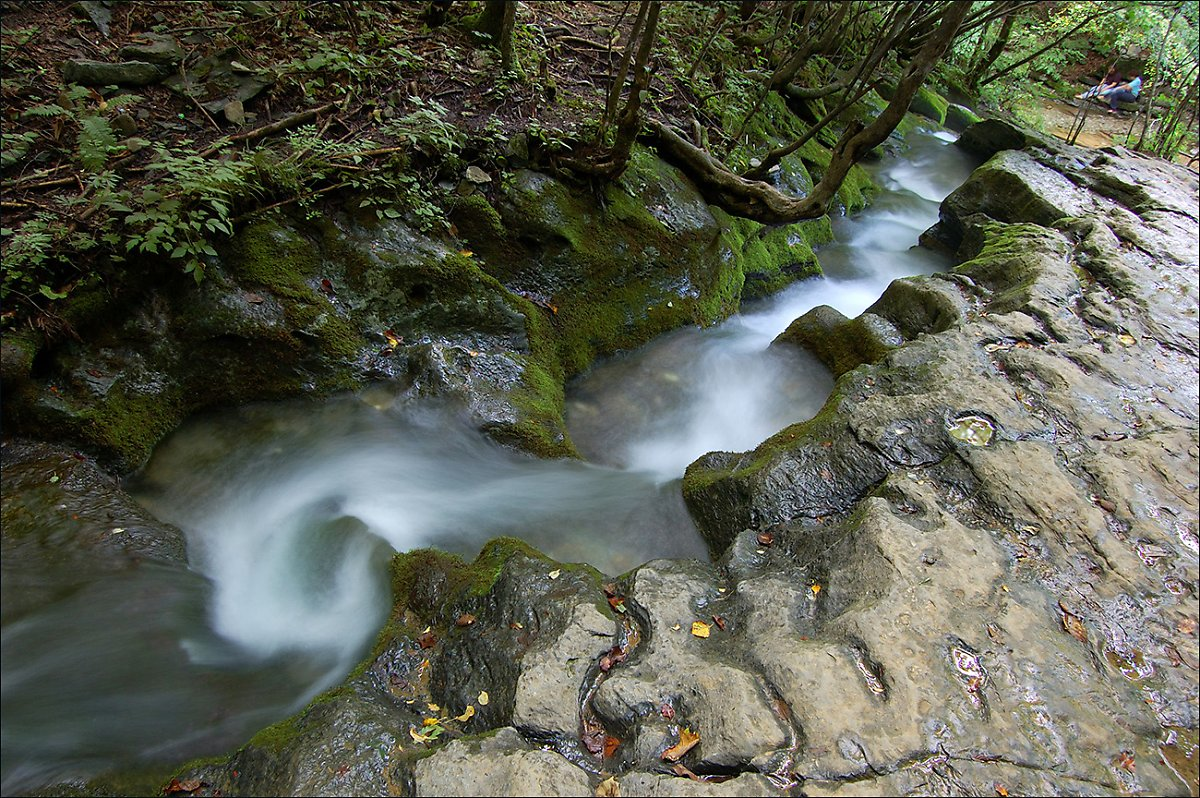
\includegraphics[width=.32\textwidth]{s_img/검룡소_사진.jpg}
    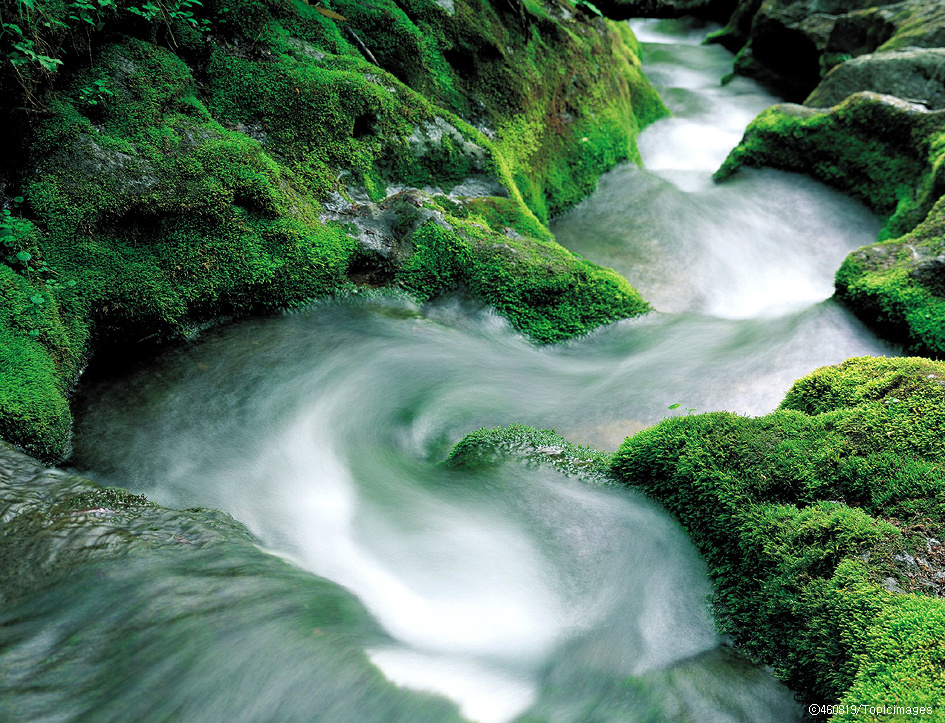
\includegraphics[width=.32\textwidth]{s_img/검룡소_사진2.jpeg}
    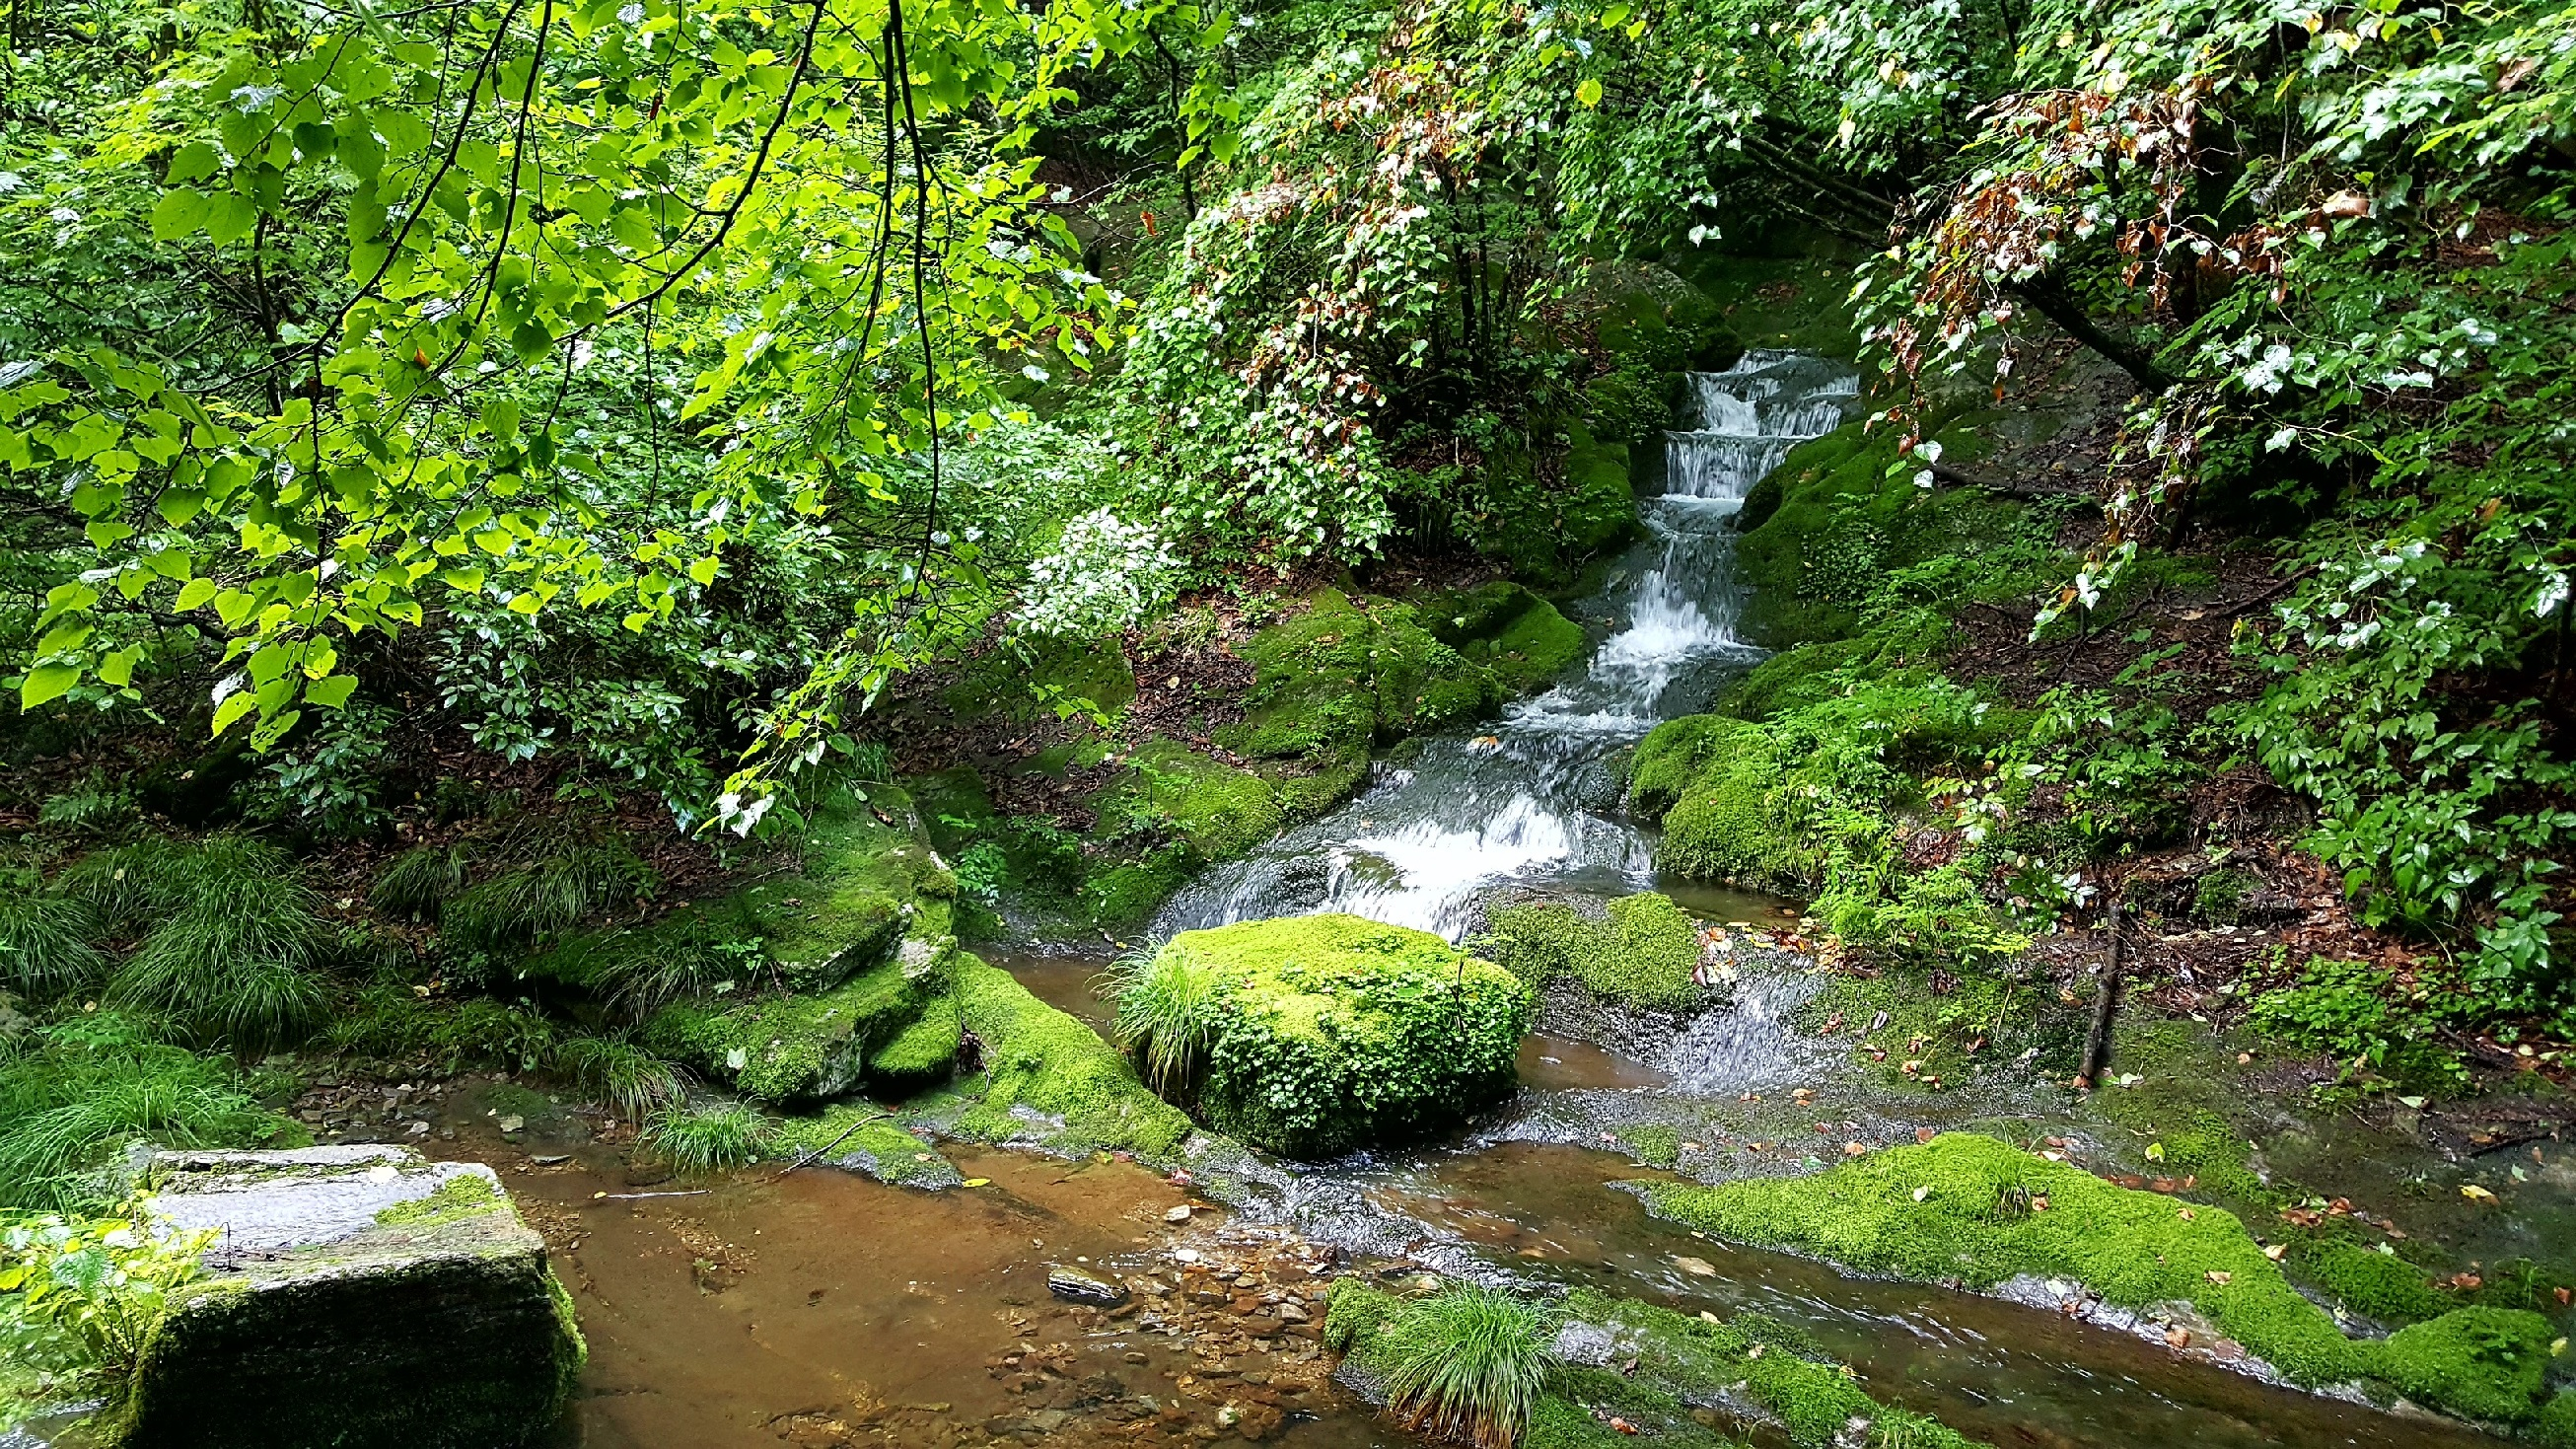
\includegraphics[width=.32\textwidth]{s_img/태백검룡소_사진_low.jpg}
    \caption{검룡소의 모습}
    \label{fig:my_label_s1}
 \end{figure}

\section{점심: 콧등치기국수 - 정선}
\subsection{메밀과 정선}
강원도 정선에서는 예로부터 메밀 농사를 많이 지었다. 
메밀은 척박한 땅에도 잘 자랐기 때문에 고추나 감자를 심고 남은 돌밭에 메밀을 심고는 했다. 
이마저도 메밀은 다른 작물과 심는 법이 달랐다. 
대개 작물을 심을 때 골을 켜고 씨앗을 심었다면, 메밀은 그저 밭에 씨앗을 뿌릴 뿐이었다. 
이곳 정선의 사람들은 그걸 `메밀을 푼다'고 했다. 메밀은 잘 자라는 것만큼이나 버릴 것 하나 없었다. 
메밀 잎은 나물로 무쳐 먹고, 줄기는 불쏘시개로 쓰기 알맞으며, 메밀 껍질 `달갱이'는 베개 속으로 사용했다.

정선의 먹을거리에는 메밀이 빠지지 않는다. 메밀국수를 비롯해 메밀묵, 메밀전병, 메밀전, 메밀국죽 등 
정선을 대표하는 메밀 먹거리들이다. 
이렇게 메밀로 만든 음식이 많음에도 메밀이 가진 고유의 맛과 모양 덕분에 매일 질리지 않고 메밀로 만든 음식을 즐길 수 있다. 

\begin{figure}[ht]
    \centering
    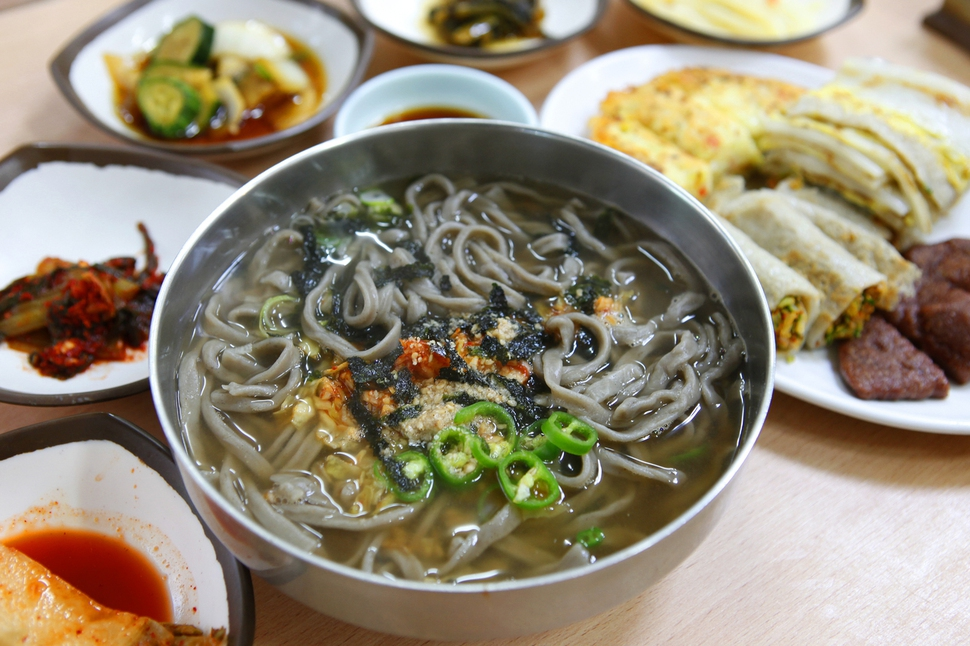
\includegraphics[width=.6\textwidth]{s_img/콧등치기국수_사진.JPG}
    \caption{콧등치기국수 사진}
    \label{fig:my_label_s2}
 \end{figure}

\subsection{메밀 국수와 콧등치기 국수}
메밀 국수를 시키면 메밀 반죽으로 만든 굵고 납작한 국수를 뜨근한 육수와 함께 준다. 
쫄깃한 면발은 고명으로 올라간 갓김치와 정말 잘 어울린다. 
그러나 정선에서 메밀 국수는 콧등치기 국수로 더 유명하다. 
정선아리랑연구소의 시인 진용선씨는 정선 문화의 대중화를 위해 메밀 국수에 콧등치기 국수라는 이름을 붙였다. 
잡지나 신문에 글을 쓸 때마다 콧등치기 국수란 말을 사용하여 요즈음에는 메밀 국수보다 콧등치기 국수란 말이 더 유명해졌다. 
메밀 국수의 다른 이름이 콧등치기 국수가 된 것은 퉁퉁한 면발이 자꾸 콧등을 친다며 붙어졌다. 


\section{조선의 불운한 왕 단종, 영월}
\subsection{삼면은 강으로 둘러쌓인 청령포}
청령포의 주변은 전형적인 감입곡류 하천의 형태를 띄고 있다. 
지반이 융기하면서 형성된 감입 곡류 하천은 측방 침식보다 하방 침식이 활발하게 나타나기 때문에 강의 폭보다는 수심이 깊은 형태를 띤다. 
또한 주변에서 하중도나 구하도, 우각호 등의 지형을 살펴볼 수 있다. 삼면이 강으로 둘러쌓여 있고, 
뒤는 암석 절벽으로 막혀 있어 청령포에 가는 방법은 오로지 배를 타고 강을 건너가는 것뿐이다. 
청령포를 둘러싼 서강이 과거 흐르던 방절리 주변 저지대에는 구하도와 곡류핵, 하안단구가 잘 보존되어 학술적으로 큰 의미가 있다.


\begin{figure}[ht]
    \centering
    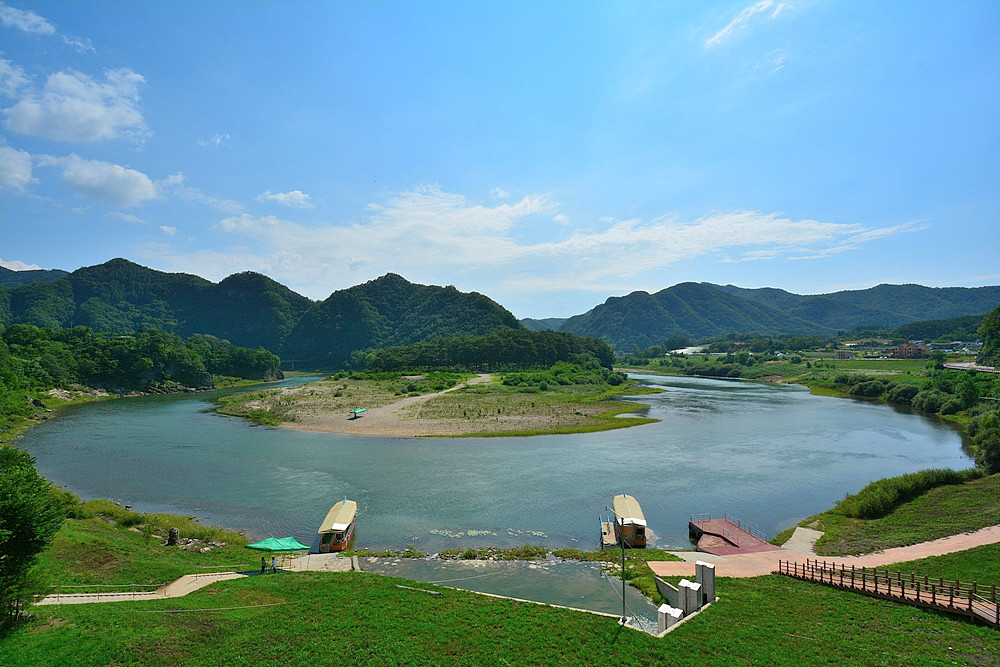
\includegraphics[width=.4\textwidth]{s_img/청령포_사진.jpeg}
    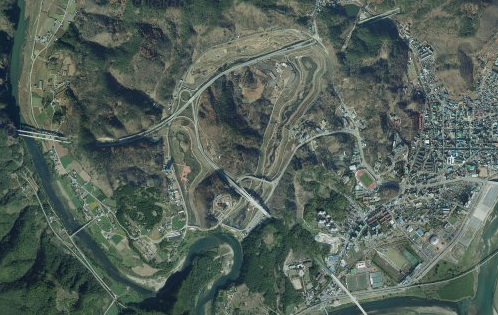
\includegraphics[width=.4\textwidth]{s_img/청령포_구하도.png}
    \caption{(좌)청령포 전경 $\quad$ (우)청령포 주위의 구하도\protect\footnotemark}
    \label{fig:my_label_s3}
 \end{figure}
 \footnotetext{\href{http://kko.to/zgW6gWkYM}{카카오맵 갈무리}}

 
\subsection{단종의 유배 생활}

앞서 설명한 바와 같이 이곳 청령포는 배를 타지 않고서는 나갈 수 없는 지형을 가지고 있다. 
이에 청령포는 1457년(세조 3년)에 단종이 세조에게 왕위를 빼앗기고 유배를 당했던 장소가 되었다. 
강나루 옆에는 단종의 유배길에 금부도사로 온 왕방연의 시비가 세워져 있다. 
당시 왕명을 수행할 수밖에 없었던 왕방연의 한없이 슬픈 마음이 비에 새겨져 있다. 
회단종이작시조(懷端宗而作時調) - ``천만리 머나먼 길에 고운님 여의옵고 내 마음 둘 데 없어 냇가에 앉았으니 저 물도 내 안과 같아서 울면서 밤길을 가더라.''
청령포 안에는 유배 당시 단종이 살았던 단종어가가 승정원일기의 기록을 토대로 복원되어 있다. 

이곳 단종어가 앞뜰에는 단종의 옛 집터를 기념하기 위해 영조 39년에 세운 비가 있다. 
비의 앞면에는 영조가 직접 하사한 ``단묘재본부시유지(端廟在本府時遺址)''라는 글이 써 있고, 
뒷면에는 ``歲皇明崇禎戊辰紀元後三癸未季秋泣涕敬書令原營竪石''라는 글이 써 있다. 
청룡포 서쪽 능선에는 망향탑이 있다. 이 망향탑은 열일곱 살 단종이 자신의 배우자 정순왕후 송 씨를 생각하며 주위에 돌을 쌓아 만든 탑이다. 
정순왕후 송 씨는 궁궐에서 쫓겨난 뒤 지금의 숭인동에 초가집을 짓고, 매일 아침저녁으로 동망봉에 올라 단종의 무사를 기원했으며, 
단종의 죽음을 알고는 매일 통곡하며 명복을 빌었다고 전해진다. 

\begin{figure}[ht]
    \centering
    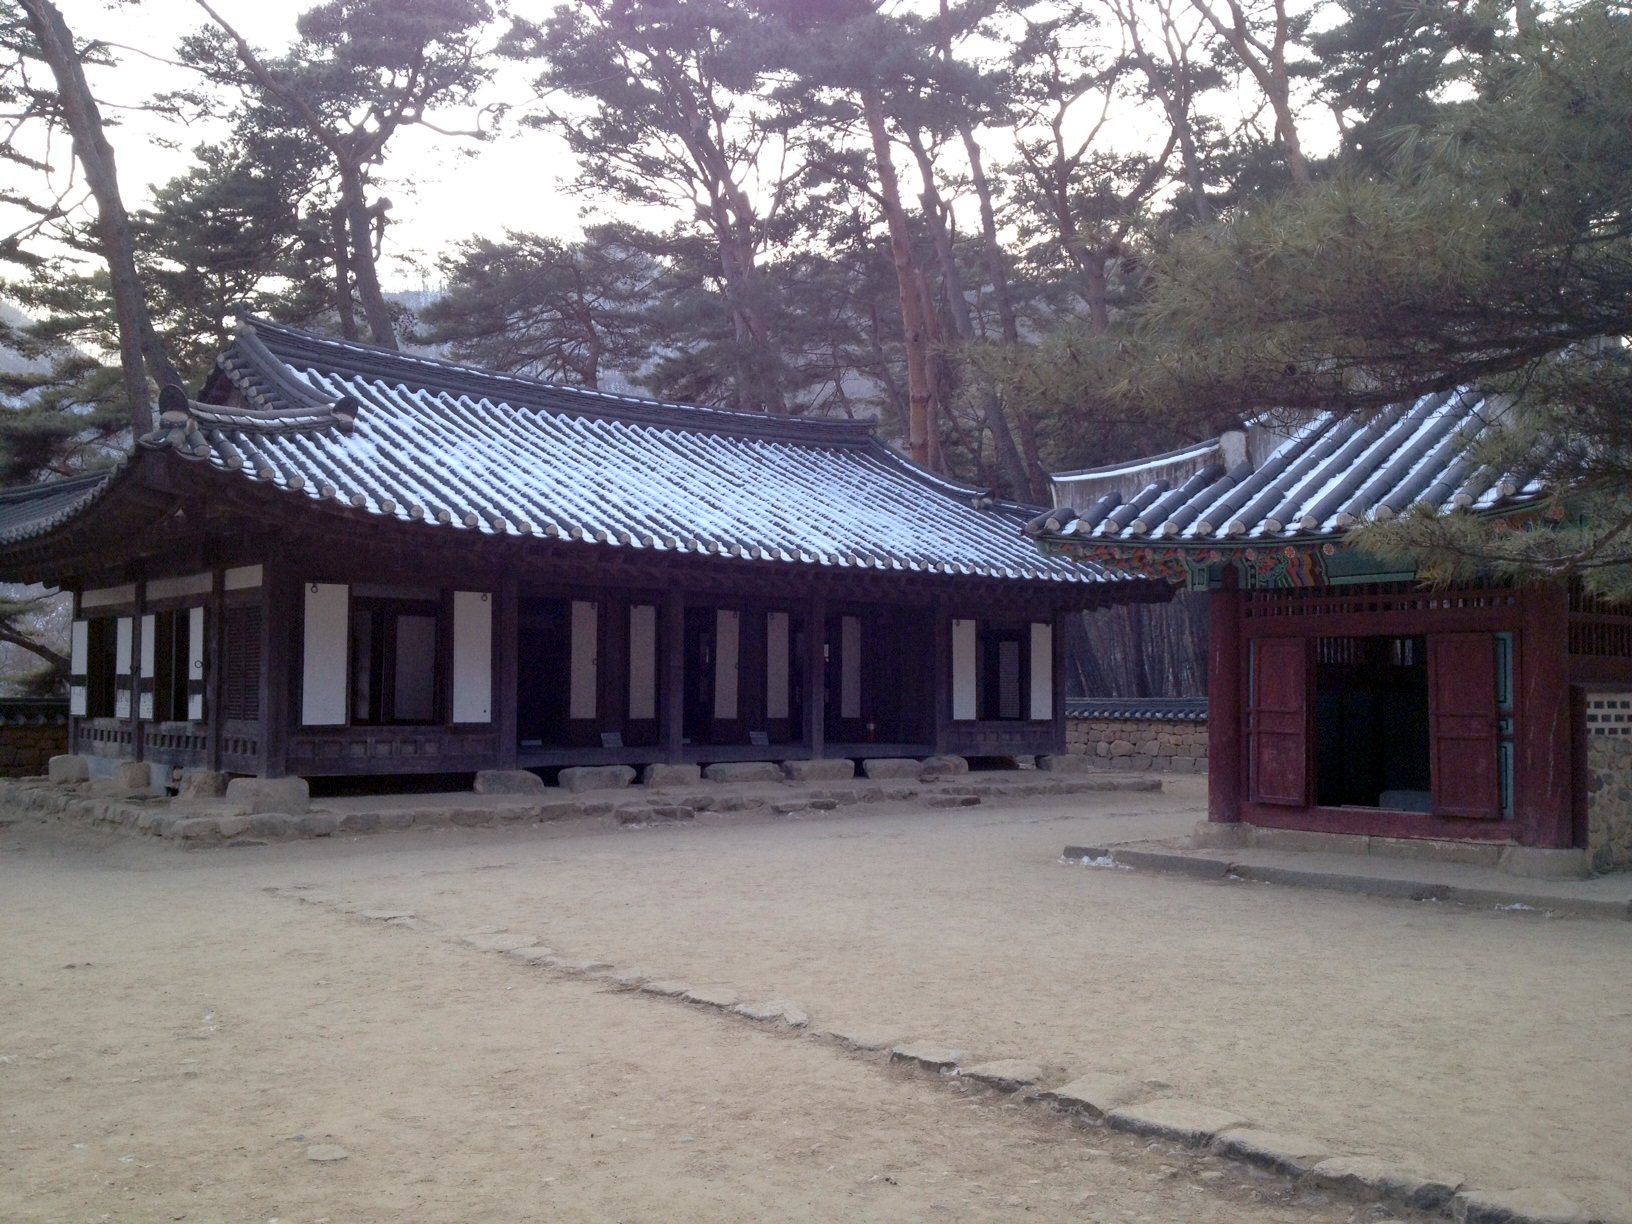
\includegraphics[width=.6\textwidth]{s_img/청령포_사진_2.JPG}
    \caption{청령포 내에 위치한 단종 어소. (단종이 유배되어 있던 곳) \protect\footnotemark}
    \label{fig:my_label_s31}
\end{figure}
\footnotetext{\href{https://commons.wikimedia.org/wiki/File:CheongRyeongpo_Eoso.JPG}{단종의 첫 유배지 청령포에 위치한 어소. $|$ 위키미디어 공용, 2012.01.11}}


\section{바보 온달과 평강 공주, 단양}
\subsection{평강 공주 전설}
고구려 평원왕의 딸이었던 평강 공주는 어려서부터 자주 울었고, 그때마다 아버지 평원왕은 바보 온달에게 시집보내겠다며 공주를 놀렸다. 
평강 공주가 16세가 되던 해에 평원왕이 공주를 상부(上部)의 고씨 가문에 시집보내려 하자, 
공주는 이를 거부하고 궁궐에서 뛰쳐나갔다. 공주는 어릴 적 귀가 빠지게 듣던 바보 온달을 찾아갔다. 
장님이었던 온달의 어머니는 찾아온 평강 공주의 향기와 부드러운 손을 만져보고는 이곳은 이렇게 귀하신 분이 오실 곳이 아니라 하였다. 
때마침 집에 온 온달마저도 어린 여자가 할 행동이 아니라며 공주를 강하게 거부했다. 
그러나 공주는 포기하지 않고 다음날 아침에 온달 모자를 다시 설득했고, 마침내 그 둘은 혼인하였다. 
평강 공주는 가져온 팔찌를 팔아 살림을 장만하고 말을 정성스레 키웠다. 그리고 그 말은 온달과 함께 전투에서 큰 공을 세웠다. 
590년, 온달은 아단성에서 신라와 싸우다 전사해 관에 들어가게 되었는데, 
그 관은 아무리 옮기려 해도 꿈적도 하지 않았다. 
이에 평강이 관을 어루만지며 이미 생사는 정해졌으니 이만 돌아가자고 하자, 그제서야 관이 움직이기 시작했다. 


\begin{figure}[ht]
    \centering
    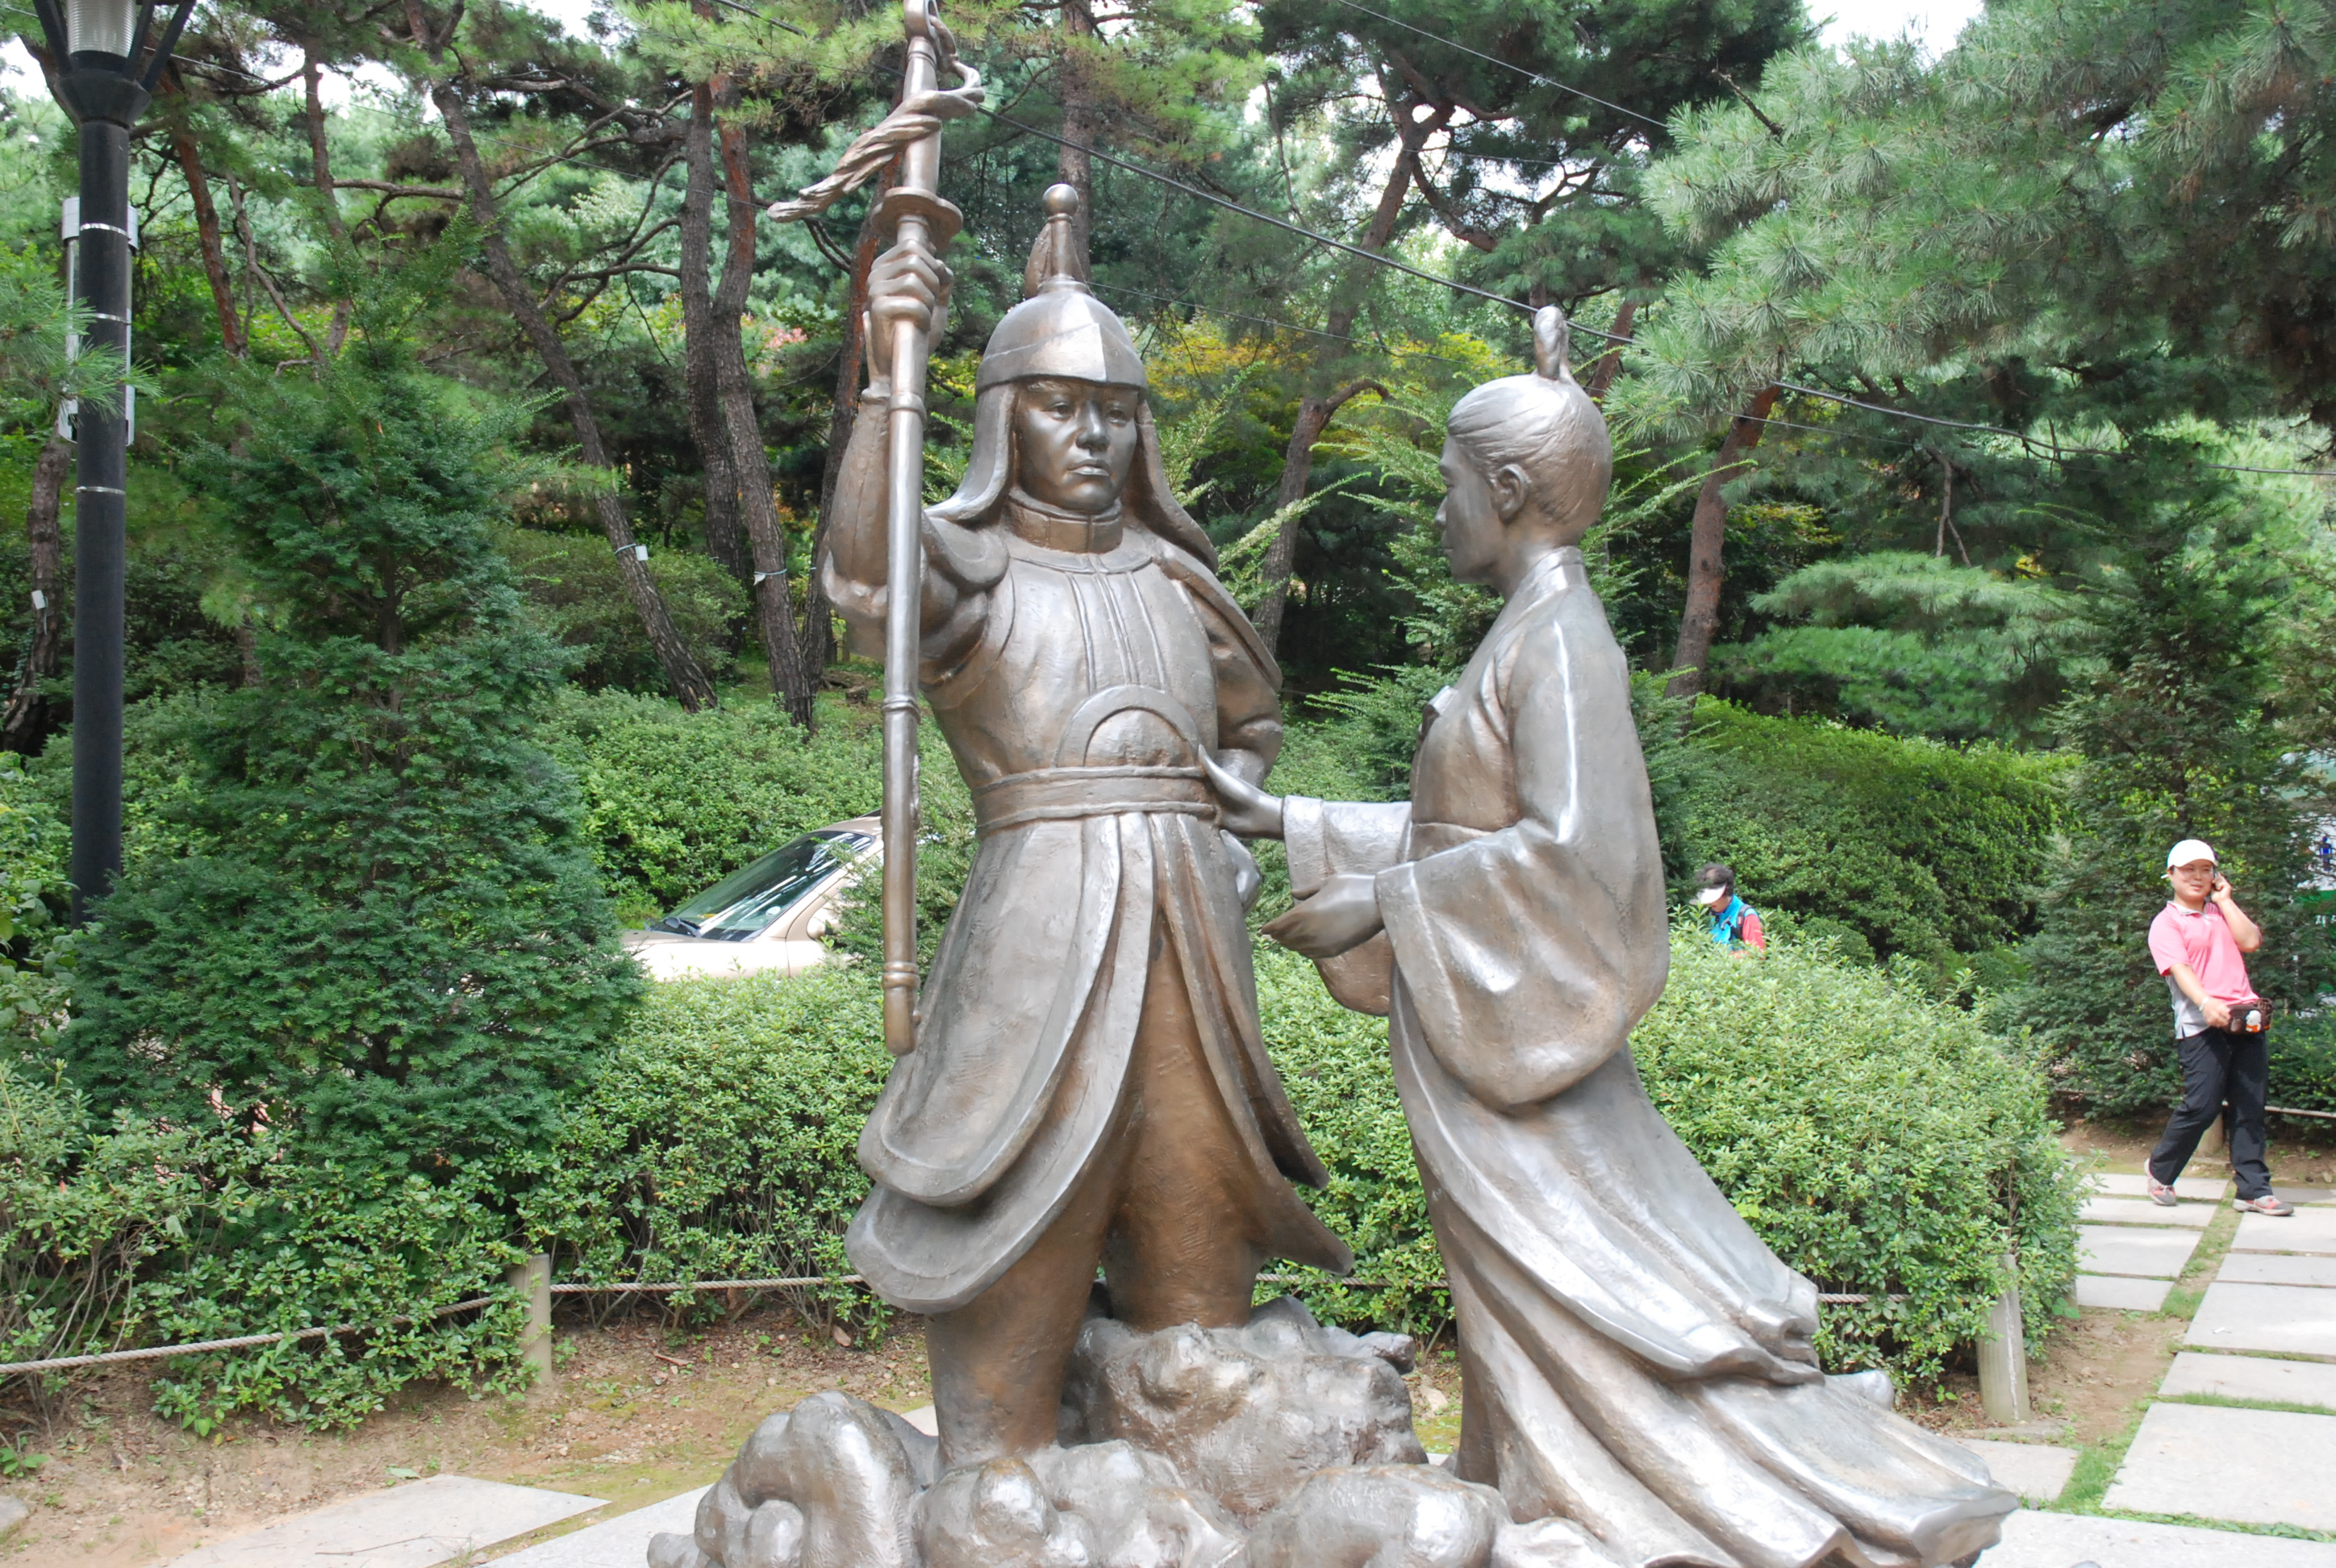
\includegraphics[width=.6\textwidth]{s_img/온달_사진.jpg}
    \caption{온달 동상의 모습}
    \label{fig:my_label_s4}
 \end{figure}

\subsection{온달 공원 탐방}
$<$연개소문$>$, $<$태왕사신기$>$, $<$바람의 나라$>$, $<$천추태후$>$ 등의 드라마가 제작된 이곳 온달 공원은 
온달 전시관을 비롯해 온달 산성, 온달 동굴 등 명승이 모여있는 곳이다. 
온달 공원 이곳 저곳에는 실제 촬영을 위해 사용된 세트장이 아직 남아있는데, 촬영에 사용된 의상이나 소품도 함께 배치되어 있어 
드라마 촬영 현장을 생동감 넘치게 즐길 수 있다. 
온달 전시관 옆에는 석회질 동굴인 온달 동굴이 있다. 
온달 동굴은 1979년 6월에 천연기념물 261호로 지정된 총길이 700m 가량의 석회동굴이다. 
이름이 온달 동굴인 까닭은 온달 장군이 쌓은 온달 산성 아래 위치해 있기 때문이다. 
이 동굴의 입구는 남한강변에 위치해 강수 등의 이유로 수위가 높아지면 동굴이 물에 잠기는 까닭에 내부에 사는 생물은 찾아볼 수 없다. 
동굴 내부는 꾸준히 물이 흐르기 때문에 단조로운 형태를 띄며 식생도 다양하지 않다. 
그러나 동굴 내부에서 석순을 어렵지 않게 찾아볼 수 있다. 


온달 산성의 다른 이름은 아단성으로 실제 온달이 신라와 싸우다 전사한 장소이다. 
성산의 정산 부근을 돌로 쌓아 만든 둘레 683m 정도의 소규모 산성으로, 
내외부에서 삼국시대 유물과 우물터, 배수구 등이 발견된다. 
한강은, 한반도의 중부를 흐르는 강으로 삼국시대 삼국의 접경지대였다. 
또한, 강 주변의 비옥한 평야지대, 수운을 이용할 수 있어 교통이 유리하고, 중국과 교역할 수 있다는 점에서 삼국이 모두 탐내는 곳이었다.
끝내 한강을 차지한 신라가 삼국을 통일했다는 점에서, 비록 결과론적이지만
한강의 지배자가 한반도의 지배자가 된 것이다.
남한강이 내려다 보이는 산자락에 위치한 온달산성은, 
이러한 삼국의 각축전을 잘 보여주는 장소이다.
\footnote{\href{https://www.edunet.net/nedu/contsvc/viewWkstCont.do?clss_id=CLSS0000000362&menu_id=81&contents_id=1d7c0c64-bc0f-45e7-8f4d-82a7bb00cc97&svc_clss_id=CLSS0000072410&contents_openapi=naverdic}
{에듀넷 T 클리어 $>$ 교과주제 학습자료 $>$ 사회 $>$ 삼국 시대와 동아시아의 재편 $>$ 삼국시대 한강 유역의 의미 $|$ 한국교육학술정보원}}


\begin{figure}[ht]
    \centering
    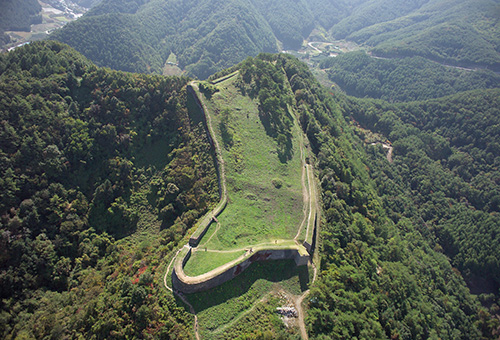
\includegraphics[width=.4\textwidth]{s_img/온달산성_사진.JPG}
    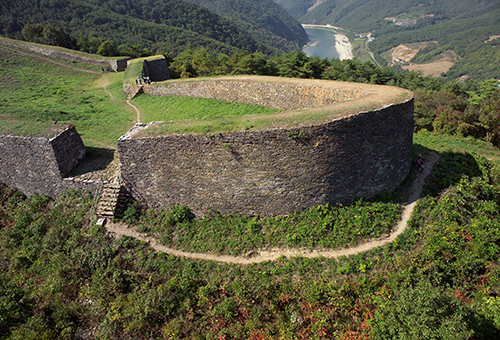
\includegraphics[width=.4\textwidth]{s_img/온달산성_사진2.JPG}
    \caption{하늘에서 본 온달산성 전경}
    \label{fig:my_label_s5}
 \end{figure}

\section{쓰라린 패배의 기억, 충주}
\subsection{충주 탄금대와 임진왜란}
충주 탄금대는 임진왜란에서 탄금대 전투가 일어난 지역으로 유명하다. 임진왜란 당시 부산진성과 동래성이 함락되고 파죽지세로 상주마저 함락되었다. 이에 선조는 신립에게 왜군 방어 임무를 내렸고, 신립은 그렇게 문경으로 출동했다. 신립과 함께한 김여물은 문경새재의 언덕과 바위를 방패 삼아 궁병으로 공격하자고 했으나, 신립은 충주의 달천 평야에서 궁기병을 활용해 공격하자고 했다. 이는 신립이 일본군의 대부분이 보병이므로, 조선의 기병이 일본을 상대로 우위를 점할 수 있을 것이라 생각했기 때문이었다. 그러나 이는 틀린 추측이었다. 달천 평야의 논밭은 젖어있어서 기병이 활동하기 어려운 지형이었고, 결국 일본군에게 참패하고 만다. 그 결과 신립은 탄금대에 몸을 던져 익사했다고 전해진다. 
